\section{Experiment 1: Helium}
\subsection{Reference line}

We placed the transmission grating at $45.71\,\text{cm}$ and the spectrometer scale at $9.13\,\text{cm}$, with the discharge tube behind the central opening. Bright first order lines appeared on both sides. A faint second order was visible at large angles, mainly in yellow. We checked alignment by comparing opposite line positions. The apparent line width was about $0.1\,\text{cm}$.

\begin{figure}[H]
\centering
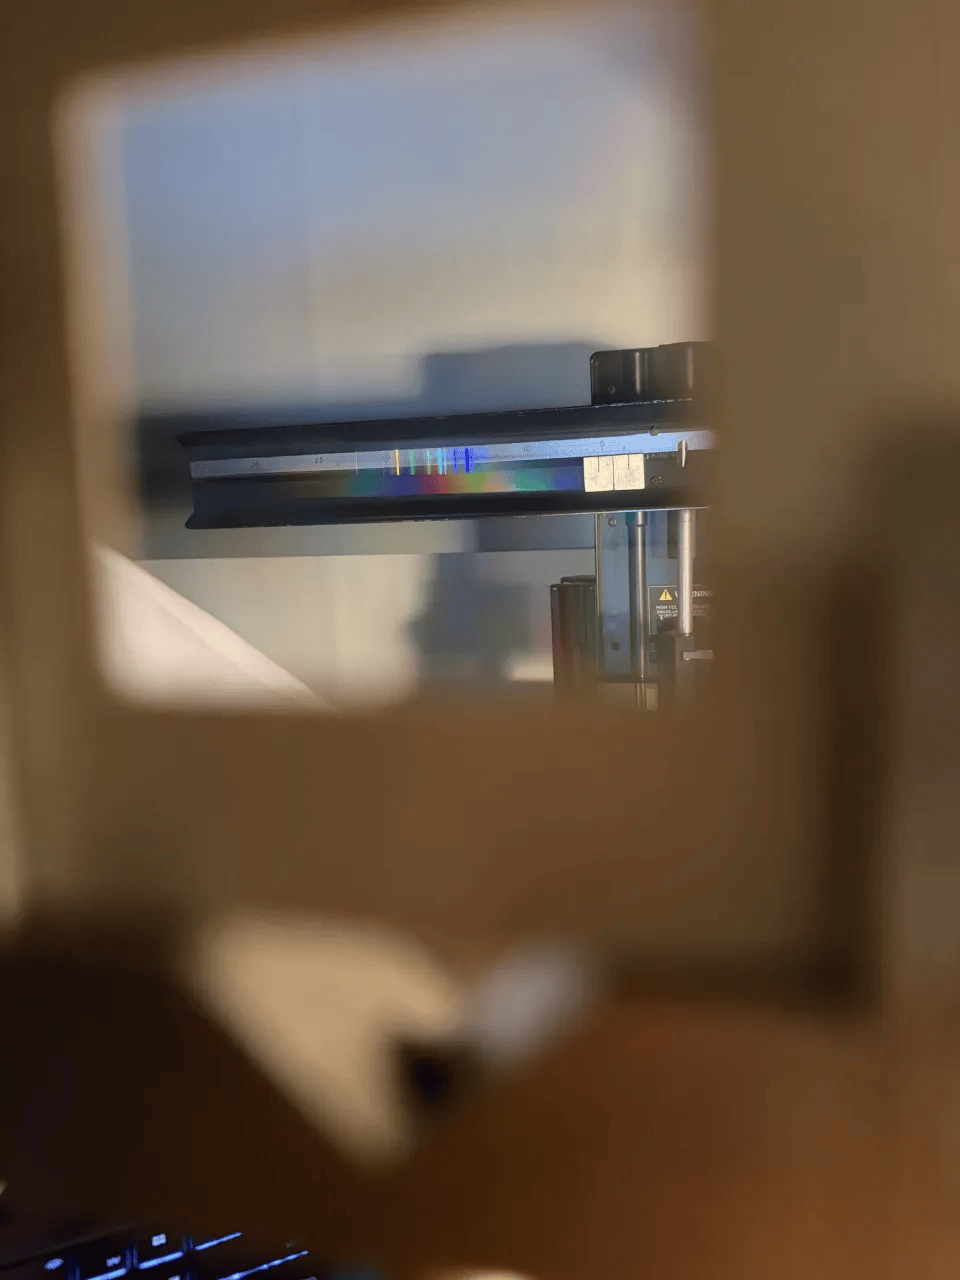
\includegraphics[width=\linewidth,trim=80bp 600bp 180bp 300bp,clip]{Photos/5CL_5_1.png}
\caption{Helium viewed through the transmission grating.}
\label{fig:helium}
\end{figure}

\begin{table}[H]
\centering
\begin{tabular}{cccc}
\toprule
Observer & Left / $\text{cm}$ & Right / $\text{cm}$ & Recorded uncertainty / $\text{cm}$ \\
\midrule
Isaac & 11.18 & 11.11 & 0.15 \\
Forrest & 11.30 & 11.30 & 0.10 \\
\bottomrule
\end{tabular}
\caption{Independent placements of the helium D3 line. The uncertainty column preserves the original estimates. Experiment 2 uses the measured scatter of these four readings.}
\label{tab:helium-repeat}
\end{table}

\clearpage
\subsection{Visible spectrum}

We recorded three additional first order lines on the right. Using the known D3 wavelength $587.6\,\text{nm}$ and the full grating geometry gives
\begin{equation}
\lambda=d\sin\theta=d\frac{y}{\sqrt{L_{He}^2+y^2}}.
\end{equation}

\begin{table}[H]
\centering
\begin{tabular}{ccc}
\toprule
Observed color & Recorded $y$ / $\text{cm}$ & Calculated $\lambda$ / $\text{nm}$ \\
\midrule
Red & $12.87\pm0.09$ & $665\pm5$ \\
Yellow (D3) & $11.22\pm0.05$ & 587.6 (reference) \\
Green & $9.51\pm0.09$ & $504\pm5$ \\
Blue & $8.46\pm0.09$ & $451\pm5$ \\
\bottomrule
\end{tabular}
\caption{Calculated helium wavelengths, with uncertainties propagated by the method in Experiment 2. The yellow offset is the mean of four placements, and its wavelength is fixed by the reference.}
\label{tab:helium-wavelength}
\end{table}

These roughly match the handout's helium lines near $668\,\text{nm}$ and $588\,\text{nm}$, together with $502\,\text{nm}$ and $447\,\text{nm}$. Strong yellow accompanied by blue and green provides a useful helium fingerprint.

The reflection grating and screen were off the bench, making distances poorly constrained. We used a small reflection angle to reduce projection effects. No additional fluorescence wavelength was recorded.

\begin{figure}[H]
\centering
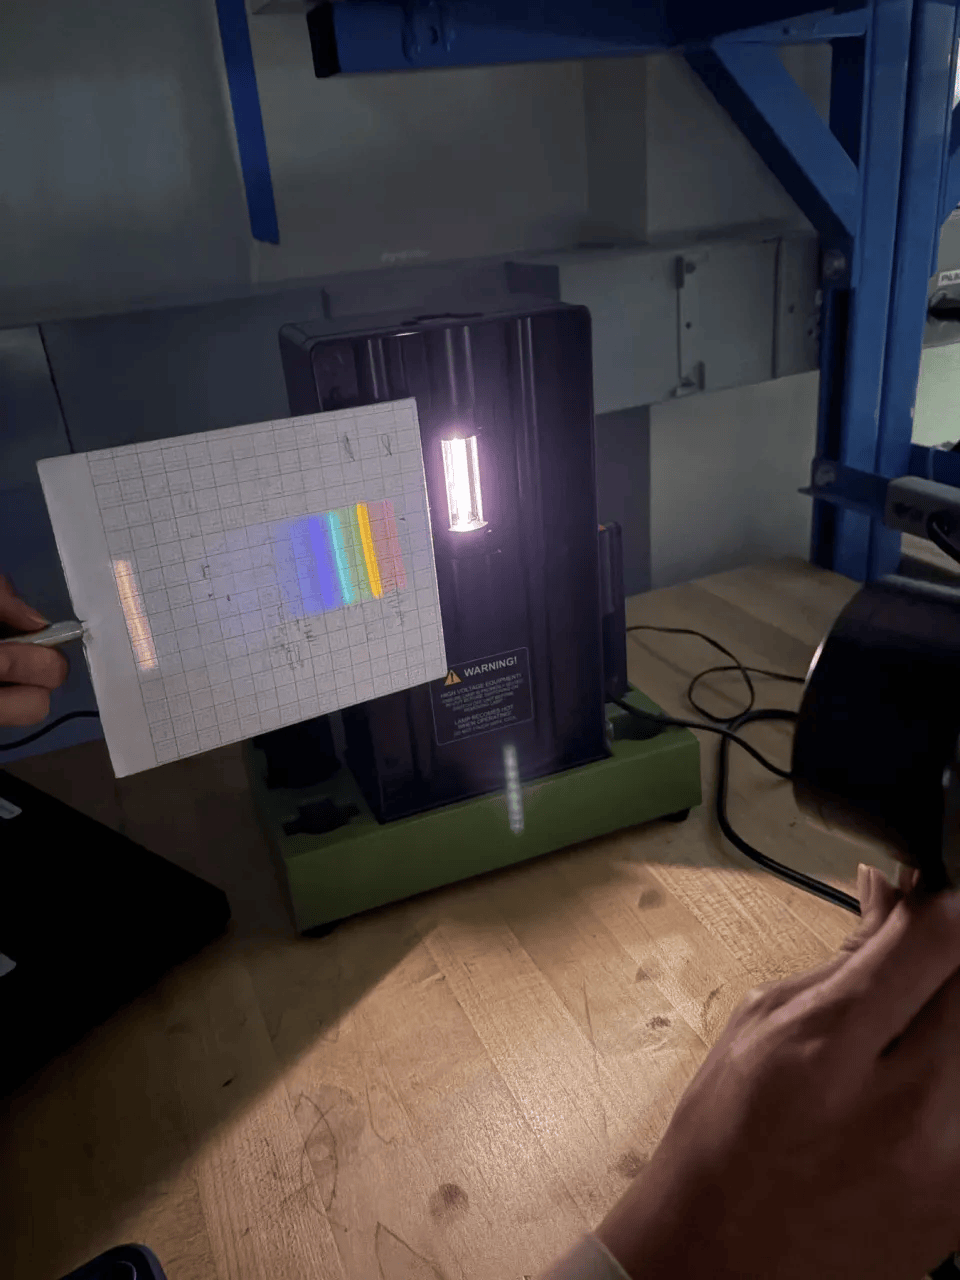
\includegraphics[width=\linewidth,trim=0bp 580bp 60bp 350bp,clip]{Photos/5CL_5_1b.png}
\caption{Helium spectrum projected onto the paper with the reflection grating.}
\label{fig:helium-mirror}
\end{figure}
